\begin{center}
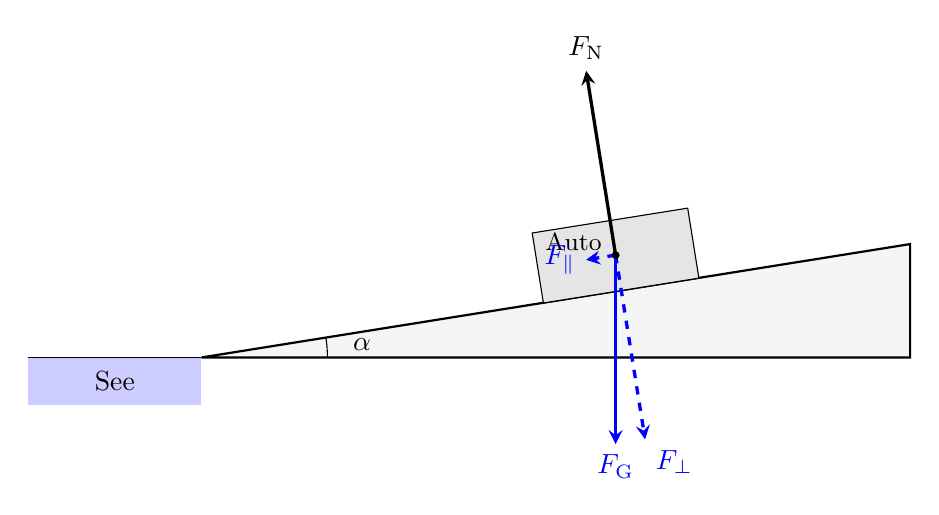
\begin{tikzpicture}[>=stealth]
 \draw[thick, fill=gray!8] (0,0) -- (9.00,0) -- (9.00,1.44) -- cycle;
 \draw (1.6,0) arc (0:9.09:1.6);
 \node at (2.04,0.16) {$\alpha$};
 \begin{scope}[shift={(5.33,0.85)}, rotate=9.09]
  \draw[fill=gray!20] (-1.0,0) rectangle (1.0,0.9);
  \node[font=\small] at (-0.50,0.70) {Auto};
 \end{scope}
 \draw[->, very thick, blue] (5.26,1.30) -- ++(-90.00:2.40) node[anchor=north] {$F_\mathrm{G}$};
 \draw[->, very thick, blue, dashed] (5.26,1.30) -- ++(-80.91:2.37) node[anchor=north west] {$F_\perp$};
 \draw[->, very thick, blue, dashed] (5.26,1.30) -- ++(189.09:0.38) node[anchor=east] {$F_\parallel$};
 \draw[->, very thick, black] (5.26,1.30) -- ++(99.09:2.37) node[anchor=south] {$F_\mathrm{N}$};
 \fill (5.26,1.30) circle (0.05);
 \fill[blue!20] (-2.2,0) rectangle (0,-0.6); \draw (-2.2,0) -- (0,0); \node at (-1.1,-0.3) {See};
\end{tikzpicture}
\end{center}

Rollwiderstand und Luftwiderstand werden vernachlässigt. Die Steigung $p = \stgO$ gibt $\tan\alpha = p$, also $\alpha = \wiF = \wi$. Das Auto wird von der Hangabtriebskraft gleichmässig beschleunigt mit
\begin{align}
 a &= \aAuF = \gE\cdot\sin\left(\wi\right) = \aAu
\end{align}
Es startet aus der Ruhe, seine mittlere Geschwindigkeit ist also die Hälfte der Endgeschwindigkeit $v = a\,t$:
\begin{align}
 s &= \frac{v}{2}\cdot t = \frac{a\,t}{2}\cdot t
\end{align}
Daraus folgt die Zeit bis zum See
\begin{align}
 t &= \tAuF \\
   &= \sqrt{\frac{2\cdot\sSt}{\aAu}} \\
   &= \tAu \approx \result{\tAuP{0}{2}}
\end{align}
und die Geschwindigkeit
\begin{align}
 v &= a\,t = \vAuF \\
   &= \aAu\cdot\tAu \\
   &= \vAu \approx \result{\vAuP{0}{2}} = \vKmP{0}{2}
\end{align}
Wegen Roll- und Luftwiderstand wäre das Auto in Wirklichkeit langsamer.
